

\section{Channel File 291 Incident}
\label{sec:crowd}

Friday July 19, 2024, CrowdStrike, a leading cybersecurity firm, released an update to its Falcon Sensor
software designed for Windows-based systems. The update, intending to enhance threat detection single-handedly,
disrupted the global IT infrastructure, causing widespread system crashes across various industries
(e.g., airlines, healthcare, and banking) \cite{crowdstrike2024falcon}. 

The outage costed fortune \textbf{500 companies approximately \$5.4 billion} in damages, after an 
estimated \textbf{8.5 million devices} were struck by the blue screen of death (BSoD) \cite{tidy_crowdstrike_outage_2024}\cite{kerner_crowdstrike_outage_2024}.

\section{Context and Background}
\label{sec:context}

CrowdStrike's Founder and CEO George Kurtz, addressed the public on live TV, stating ``That we're deeply sorry for the impact we've caused'' \cite{sato_crowdstrike_ceo_2024}.
Though this isn't the first time George Kurtz has been caught in the crossfire of a cybersecurity incident.
In 2019, George Kurts the customer-facing Field Chief Technology Officer at McAfee, released a faulty update.
The update, mistakenly identified a critical Windows system file (svchost.exe) as malware, causing the system to endlessly loop \cite{volenik_crowdstrike_ceo_2024}.

In a blog posted by CrowdSTrike ``as of 8:00 p.m. EDT on July 29, 2024, ~99\% of Windows sensors were back online'' \cite{crowdstrike_channel_file_291_2024}.
The incident was said to occur due to a bug which expected 20 input fields instead of 21, causing the software to crash. Channel File 291 was identified the 
culprit and was removed from the software \cite{crowdstrike_channel_file_291_2024}.

\section{Modern Endpoint Security}
\label{sec:falcon}

First we will break down what exactly the Falcon Sensor is. The Falcon Sensor claims to be a lightweight agent installed on endpoint devices to monitor and record system activity.
Ensuring \textbf{endpoints} means ensuring devices that connect to a network, such as laptops, desktops, and mobile devices. \textbf{Endpoint security} is the process of 
securing the various points at which a device connects to a network. 90\% of successful breaches and 70\% of data breaches originate at endpoint,
costing companies millions \cite{ibm_endpoint_security}. 

Since many large scale companies have moved to the cloud, and many working from home, ever more devices are connecting to sensitive data. This means many endpoint solutions 
constantly monitor and record system activity to detect and prevent threats. This in itself utilizes cloud-based systems to access threat intelligence, providing autonomous 
real-time protection \cite{cisco_endpoint_security}

Many original anti-viruses signature based, protecting endpoints on a device by scanning for known malware---\textbf{Indicators of Attack (IOA)}. 
This relied on a database of known malware signatures. CrowdStrike and many others
have opted to use \textbf{next-gen anti-virus (NGAV)} machine learning Technology,
to aid in detecting newer types of IOA vectors that are often fileless, by monitoring system memory  \cite{ionescu_kernel_access_2024}.

\newpage

\section{EPP \& EDR Anti-virus Solutions}
\textbf{Endpoint Protection Platforms (EPP)} like CrowdStrike may include the following features as defined by IBM \cite{ibm_endpoint_security}:
\begin{itemize}
    \item \textbf{Web control and content filtering}: protects against malicious code in websites and 
    user downloaded content. While providing a whitelist of approved websites.
    \item \textbf{Data classification and data loss prevention (DLP)}: identifies and classifies sensitive data, 
    preventing unauthorized access and data loss.
    \item \textbf{Firewall}: monitors and controls incoming and outgoing network traffic based on configured security rules.
    \item \textbf{Email Gateway}: scans incoming email attachments and links for malicious content.
    \item \textbf{Application control}: restricts the programs that users can run on their devices.
\end{itemize}

CrowdStrike's \textbf{Endpoint Detection and Response (EDR)} solution Falcon Sensor, part of the Falcon Platform, is at the root of the issue.
EDRs are a class of security tools that go beyond known threats, to monitor files entering and applications running on a system.
These \textbf{Correlate Indicators of Compromise (IOC)} systems, aggregate data from various sources---network traffic, unusual user behavior,
inconsistent permissions, system configuration changes, unverified software or domains, repetitive file access, and more \cite{microsoft_ioc}.

These systems aren't just designed to detect threats, but respond to them while an attack is in progress. This incurs IOCs many log based solutions such as 
\textbf{extended detection and response (XDR)}, and \textbf{security information and event management (SIEM)} systems to mitigate and isolate threats, going 
as far as to shut down a system if necessary. These systems typically rely on AI to establish a baseline of normal activity and detect deviations from it \cite{microsoft_ioc}.

\section{CrowdStrike Falcon Sensor Distinctions}

The immediate reason why CrowdStrike's Falcon Sensor update caused such a widespread outage was due to
the software living on at kernel level. These differ from traditional user-mode applications that crash in isolation.
Kernel-level applications are more privileged living at the heart of the operating system---if it crashes, the whole system crashes. 
This process is known as \textbf{kernel panic}, which stops the system from potentially corrupting beyond repair \cite{awati_kernel_panic}.

CrowdStrike notes three main kernel-level component features that it complies with from the Microsoft's anti-virus kernel APIs \cite{ionescu_kernel_access_2024}:
\begin{itemize}
    \item \textbf{Kernel Patch Protection (KPP)}: also known as \textbf{PatchGuard}, prevents third-party software from modifying the Windows kernel.
    Available on 64-bit (x64) Window systems, but by-passable on 32-bit (x86) systems, CrowdStrike opts to never patch the kernel. Other 
    anti-virus choose this route, which can lead to system instability if not done correctly \cite{wikipedia_kpp}.
    \item \textbf{Kernel-Mode Code Signing (KMCS)}: CrowdStrike complies with Microsoft's KMCS requirements, which ensures that all kernel-mode code obtains a
    \textbf{Extended Validation (EV) Code Signing Certificate} from a trusted \textbf{Certificate Authority (CA)} \cite{microsoft_kmcs}\cite{reasonlabs_kernel_hooking}.
    \item \textbf{Object Callbacks:} a feature that allows CrowdStrike to subscribe to various kernel events, such as file creation, registry access, and network activity.
    Instead of \textbf{kernel hooking}, which intercepts system calls \cite{microsoft_obregistercallbacks}.
\end{itemize}

CrowdStrike further justifies its kernel presence to protect against for \textbf{Early Boot Protection (EBP)} and which 
Microsoft supports with its \textbf{Early Launch Anti-Malware (ELAM)} driver \cite{ionescu_kernel_access_2024}. This protects against rootkits, which are 
malware that can hide from the operating system, by loading before the operating system itself. Having this 
protection in place, stops attackers from sticking USBs into airport kiosks or hotel computers \cite{baker_rootkits_2023}.

\section{Faulty Code and Production Updates:}

Despite CrowdStrike Falcon Sensor passing \textbf{Windows Hardware Compatibility Program (WHCP)} certifications, and 
validations through \textbf{Windows Hardware Lab Kit (HLK)} testing, the update still slipped through \cite{microsoftwhcpcertification}.
However, anti-virus software only needs to pass the WHCP and HLK tests once. They only certify that the driver running on the system 
is stable. Once the driver is installed, CrowdStrike can push updates---\textbf{without re-certification}---in a cloud-based process they call 
\textbf{Rapid Response Content (RRC)} \cite{crowdstrikechannelfile291rca}.

This process entirely relies on CrowdStrike's internal deploy and testing pipelines. CrowdStrike's testing negligence, did not thoroughly test the update,
during their RRC update to its Falcon Sensor software. Typically a software companies employ \textbf{Continuous Integration/Continuous Deployment (CI/CD)} pipelines
to catch these issues. CI/CD pipelines are characterized by multiple rounds of manual written tests, peer reviewed code, and automated stress testing to ensure the software compiles safely before deployment \cite{redhat_cicd_2023}.
These tests comprise of \textbf{unit tests}, \textbf{integration tests}, and \textbf{end-to-end (E2E) tests} to ensure the software is functioning as expected. 
Unit tests test individual components of the software, integration tests test how the components interact, and E2E, running the application in production-like environments (e.g., test and development environments before production) in 
a suite of integration tests to ensure stability. CrowdStrike lacked the CI/CD security to catch Channel File 291, a bug that effectively threw an out-of-bounds error.

\section{CrowdStrike Incident Report}

Before jumping into CrowdStrike's incident analysis, we must first understand the technical terms used in the analysis \cite{crowdstrikechannelfile291rca}:

\begin{enumerate}
     \item \textbf{Falcon OverWatch\textsuperscript{\textregistered} and Falcon Complete\textsuperscript{\texttrademark}}: OverWatch is a 24/7 managed threat hunting service led by human 
     intelligence. Complete is a \textbf{managed detection and response (MDR)} service, which is a suite of tools and services including OverWatch, to detect and remediate threats
     \cite{cosive_falcon_complete}\cite{crowdstrike_falcon_complete}\cite{crowdstrike_overwatch}.
     
     \item \textbf{Security Telemetry \& Graph Store}: Telemetry is the aggregation of data from various sources (e.g., endpoints, servers, network devices) \cite{proofpoint_telemetry}. These analytics are
     are stored locally on the Falcon Sensor's sensors in a graph database. Graph databases store information in nodes and edges to represent 
     the relationship between data points \cite{oracle_graph_database}.

     \newpage
     Falcon Sensor's interprets relationships in flowing memory to detect possible IOAs.\\
     \begin{figure}[h!]
        \vspace{-1em}
        \centering
        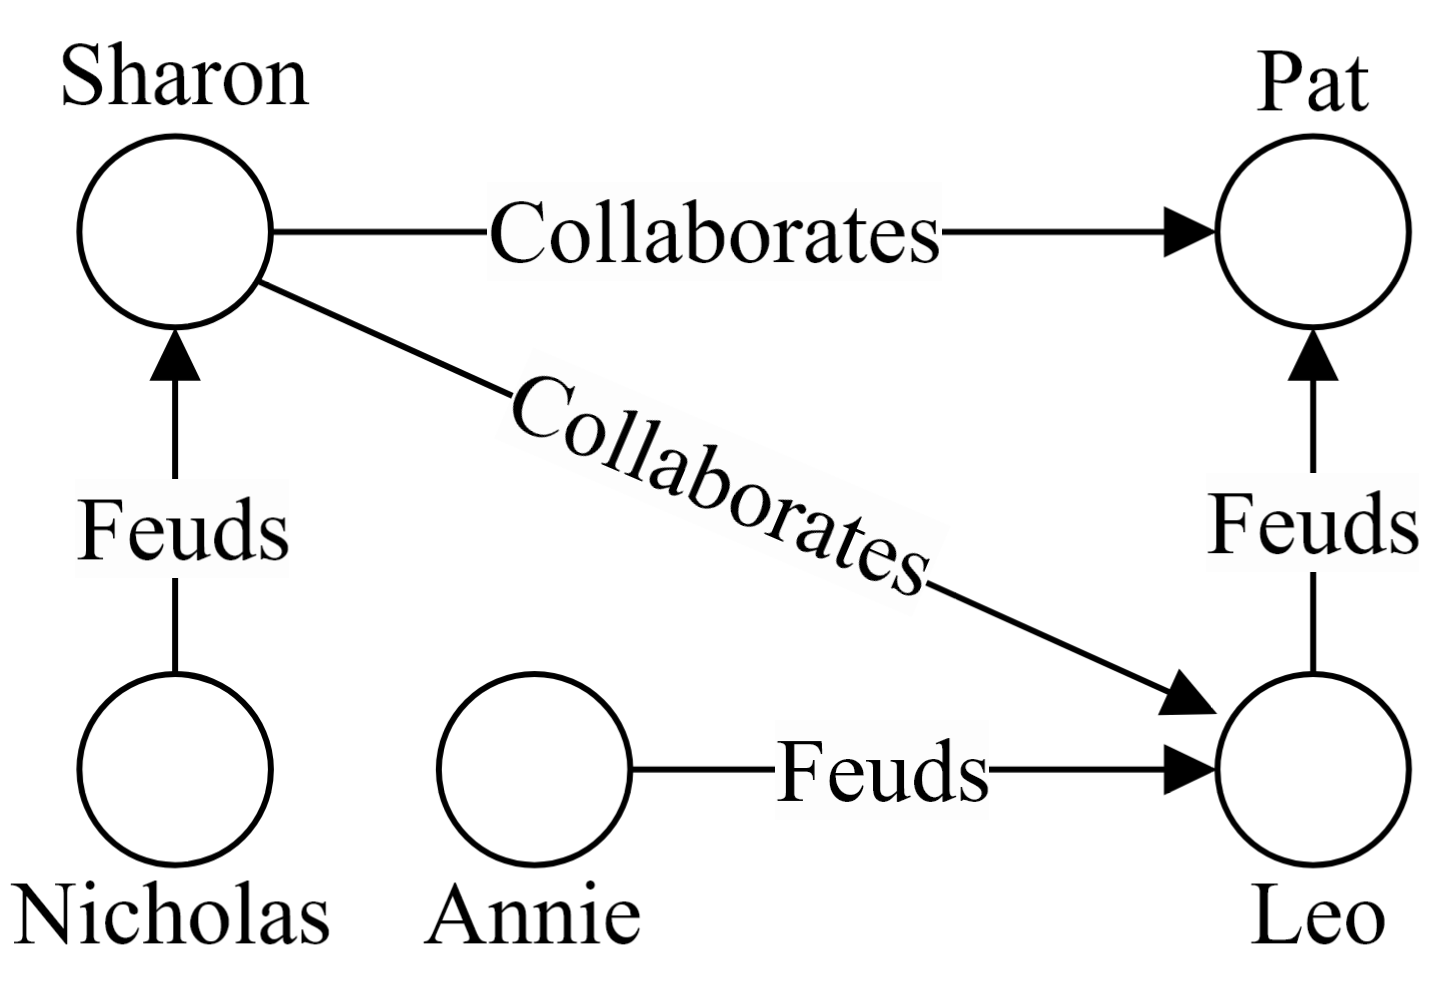
\includegraphics[width=0.35\textwidth]{Sections/crowd/graph.png}
        \caption{Graph Example Depicting Relationships Between Co-workers}
        \label{fig:graphdb}
        
        \vspace{-1em}
    \end{figure}
    
    \item \textbf{Template Types}: Template types push telemetry data to a regular-expression (RegEx) engine
    Content Interpreter. Template types outline predefined schemas of security criteria to evaluate. \textbf{Template Instances}
    are live configurations, defining parameters, thresholds, and conditions to trigger alerts.
    \item \textbf{Channel Files}: Each Falcon sensor defines a channel file, which is configured with a 
    template type. RRCs then push threat intelligence to channel files. Template instances then compare the security telemetry to 
    determine IOAs.

   
    \begin{figure}[h!]
        \centering
        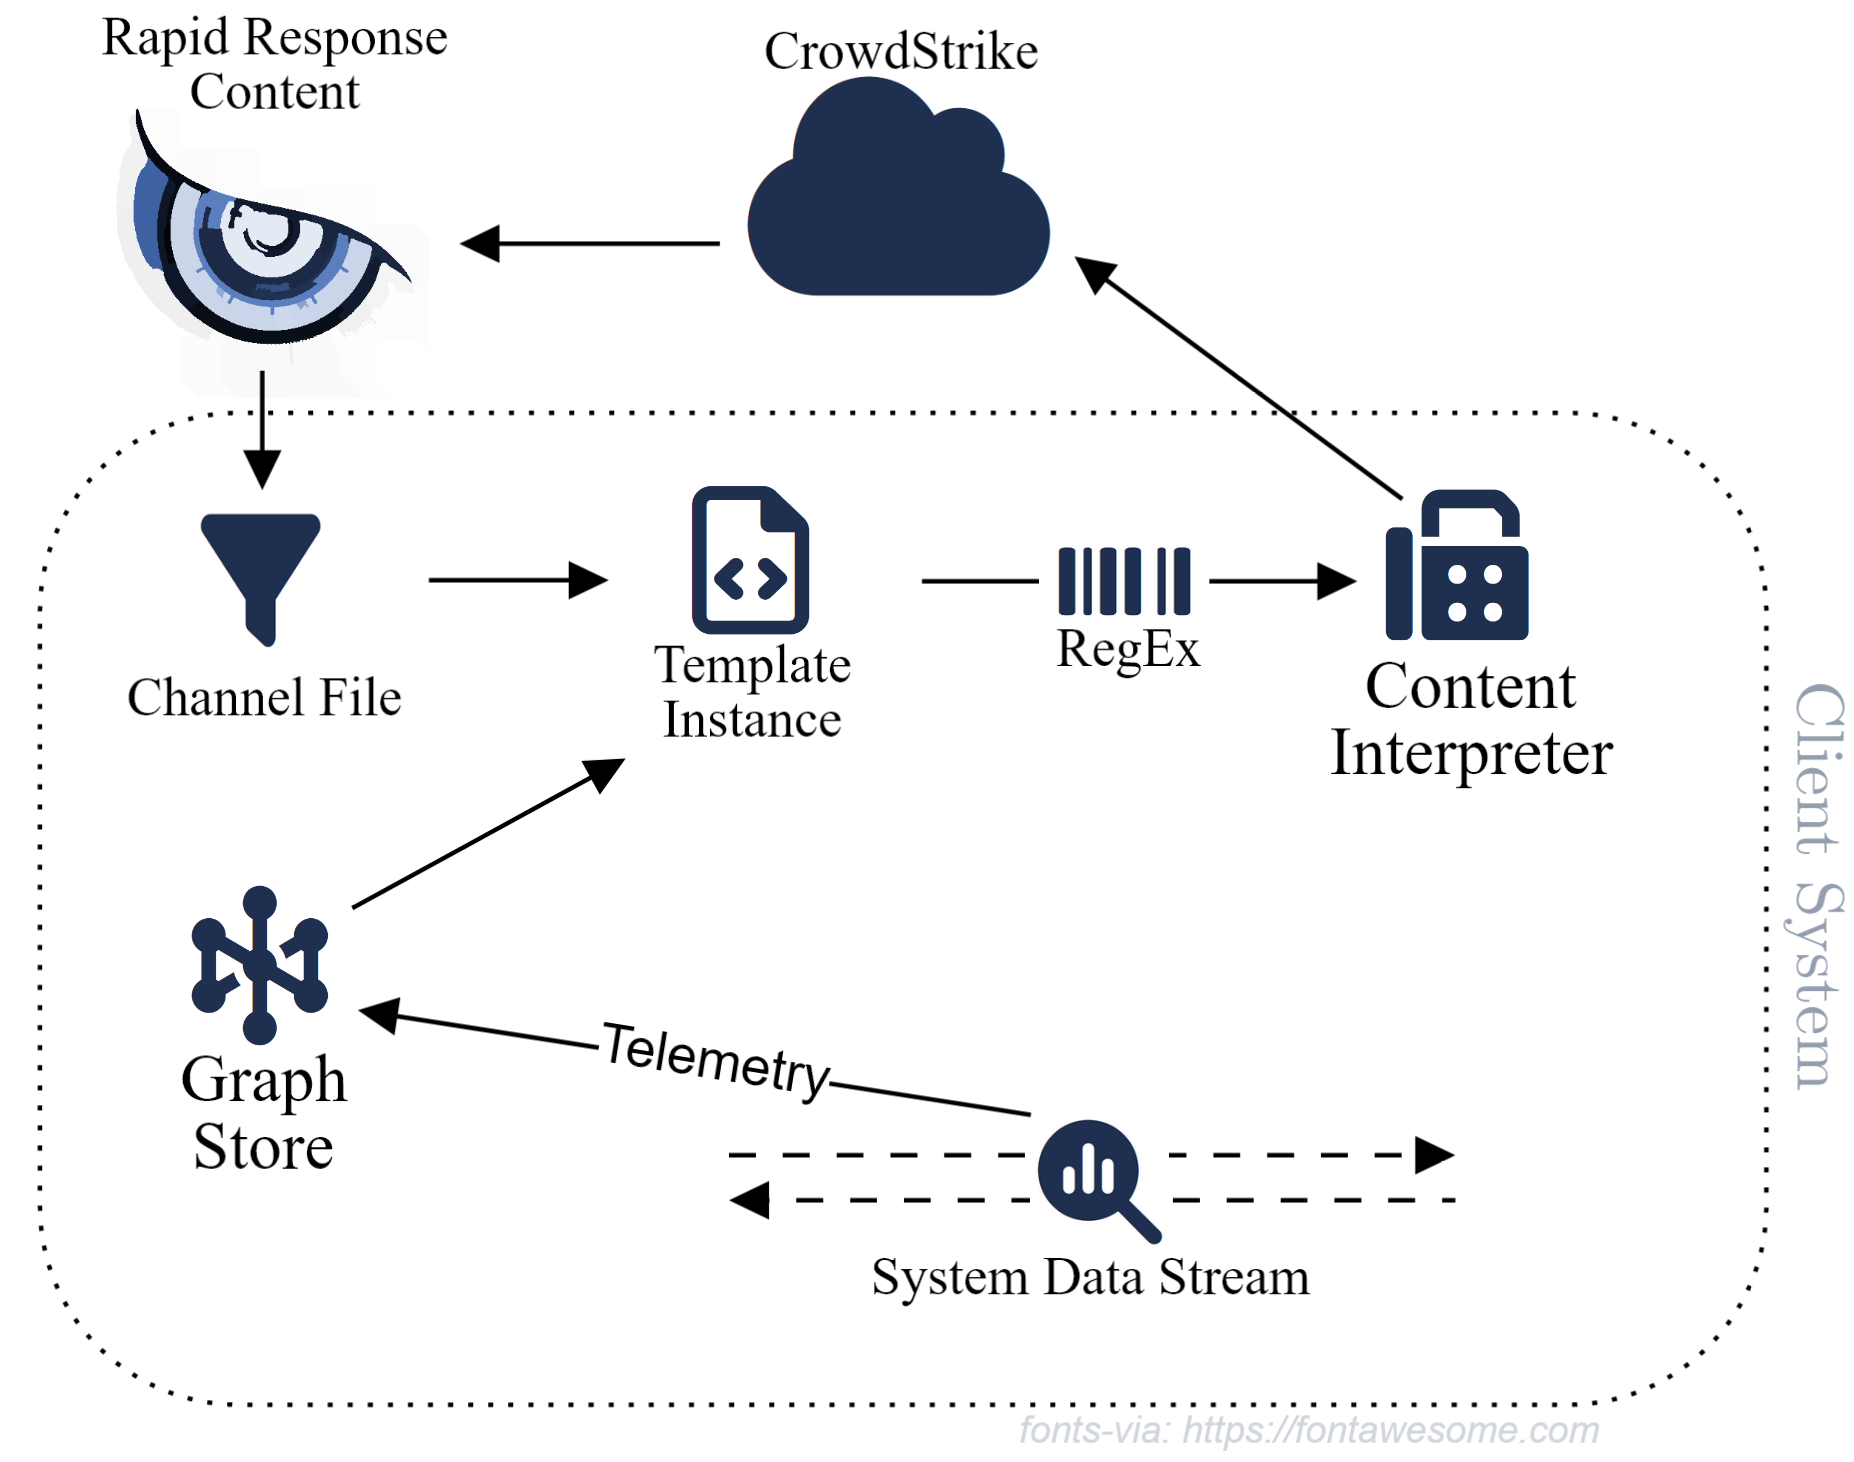
\includegraphics[width=.65\textwidth]{Sections/crowd/rrc.png}
        \caption{RRC \& Telemetry Graph Store Data Aggregation for IOA Content Interpreter.}
        \label{fig:channelfile}
    \end{figure}
\end{enumerate}

\vspace{-1em}
February 2024, CrowdStrike released sensor version 7.11, introducing a new template type.
The template type target a new IOA vector relating to \textbf{Windows Interprocess Communication (IPC)} mechanisms---notably \textbf{Named Pipes}.
Named pipes facilitate communication between processes on the same or different machines.
The exploit enabled an adversary to execute code and impersonation leading to privilege escalation \cite{sandker_named_pipes_2021}.

This release included a new IPC template type. RRC delivers IPC template instances to \textbf{Channel File 291}. This 
new template type defined 21 input fields, while the Content Interpreter still expected 20. This evaded detection 
as the Content Interpreter identified files based on a wildcard matching pattern.

\begin{lstlisting}[caption=Wildcard Pattern Matching Example]
    *: Matches any sequence 
    ?: Matches any single character
    Input: txt = ``abcdef'', pattern = ``a?c*''
    Output: true
    Reason: `?' matches with `b' and `*' matches with ``def''.
\end{lstlisting}
    
\noindent
(As CrowdStrike has mentioned their use of RegEx before, it is likely that the Content Interpreter used a RegEx pattern to match fields.)

On July 19, 2024, the RRC push two new IPC template instances to Channel---one of which dropped wildcard matching.
This required the Content Interpreter to check the 21st field from Channel File 291. However, the Content Interpreter
expected 20 fields, causing an out-of-bounds error, crashing the Falcon Sensor. This error 
caused the BSoD that Friday afternoon affecting 8.5 million devices.

\section{Windows Kernel Crash Dump Analysis}

David Weston, Vice President, Enterprise and OS Security at Microsoft, \href{https://www.microsoft.com/en-us/security/blog/2024/07/27/windows-security-best-practices-for-integrating-and-managing-security-tools/}{posted} in an incident
the kernel crash dump from Channel File 291 \cite{weston_windows_security_2024}. The Microsoft team's \textbf{Windows Error Reporting (WER)}
kernel crash dumps analysis involved \textbf{WinDBG Kernel Debugger}, and several other freely accessible debugging extensions. 

\vfill
\begin{center}
\textit{Code Dump Continued on Next Page.}
\end{center}
\vfill

\newpage

\label{sec:windbg}
\begin{lstlisting}[caption=WinDBG Kernel Crash Dump, numbers=left]
FAULTING_THREAD:  ffffe402fe868040
READ_ADDRESS:  ffff840500000074 Paged pool
MM_INTERNAL_CODE:  2
IMAGE_NAME:  csagent.sys
MODULE_NAME: csagent
FAULTING_MODULE: fffff80671430000 csagent
PROCESS_NAME:  System
 
TRAP_FRAME:  ffff94058305ec20 -- (.trap 0xffff94058305ec20)
.trap 0xffff94058305ec20
NOTE: The trap frame does not contain all registers.
Some register values may be zeroed or incorrect.
rax=ffff94058305f200 rbx=0000000000000000 rcx=0000000000000003
rdx=ffff94058305f1d0 rsi=0000000000000000 rdi=0000000000000000
rip=fffff806715114ed rsp=ffff94058305edb0 rbp=ffff94058305eeb0
 r8=ffff840500000074  r9=0000000000000000 r10=0000000000000000
r11=0000000000000014 r12=0000000000000000 r13=0000000000000000
r14=0000000000000000 r15=0000000000000000
iopl=0         nv up ei ng nz na po nc
csagent+0xe14ed:
fffff806`715114ed 458b08 mov r9d,dword ptr [r8] ds:ffff8405`00000074=???... 
.trap
Resetting default scope
 
STACK_TEXT:  
ffff9405`8305e9f8 fffff806`5388c1e4...: nt!KeBugCheckEx 
ffff9405`8305ea00 fffff806`53662d8c...: nt!MiSystemFault+0x1fcf94  
ffff9405`8305eb00 fffff806`53827529...: nt!MmAccessFault+0x29c 
ffff9405`8305ec20 fffff806`715114ed...: nt!KiPageFault+0x369 
ffff9405`8305edb0 fffff806`714e709e...: csagent+0xe14ed
ffff9405`8305ef50 fffff806`714e8335...: csagent+0xb709e
ffff9405`8305f080 fffff806`717220c7...: csagent+0xb8335
ffff9405`8305f1b0 fffff806`7171ec44...: csagent+0x2f20c7
ffff9405`8305f430 fffff806`71497a31...: csagent+0x2eec44
ffff9405`8305f5f0 fffff806`71496aee...: csagent+0x67a31
ffff9405`8305f760 fffff806`7149685b...: csagent+0x66aee
ffff9405`8305f7d0 fffff806`715399ea...: csagent+0x6685b
ffff9405`8305f850 fffff806`7148efbb...: csagent+0x1099ea
ffff9405`8305f980 fffff806`7148edd7...: csagent+0x5efbb
ffff9405`8305fac0 fffff806`7152e681...: csagent+0x5edd7
ffff9405`8305faf0 fffff806`53707287...: csagent+0xfe681
ffff9405`8305fb30 fffff806`5381b8e4...: nt!PspSystemThreadStartup+0x57 
ffff9405`8305fb80 00000000`00000000...: nt!KiStartSystemThread+0x34 
\end{lstlisting}

\begin{center}
    \texttt{[Modified to fit page with '...' usage.]}
\end{center}

\newpage

\noindent
WER shows a compressed crash dump view, so prior calls leading to the crash aren't shown.

\begin{lstlisting}[caption=Debugging csagent.sys Module (\# comments), numbers=left]
6: kd> .trap 0xffff94058305ec20 # user debugging command
.trap 0xffff94058305ec20
# Displays the CPU's register states at the time of the crash.

NOTE: The trap frame does not contain all registers.
Some register values may be zeroed or incorrect.
rax=ffff94058305f200 rbx=0000000000000000 rcx=0000000000000003
rdx=ffff94058305f1d0 rsi=0000000000000000 rdi=0000000000000000
rip=fffff806715114ed rsp=ffff94058305edb0 rbp=ffff94058305eeb0
r8=ffff840500000074  r9=0000000000000000 r10=0000000000000000
# `rip`: Faulting instruction pointer address.
# `r8`: Address being accessed; points to `ffff840500000074' (invalid memory).

csagent+0xe14ed:
fffff806`715114ed 458b08 mov r9d,dword ptr [r8]
# Faulting instruction: attempts to read a 32-bit value from address stored in `r8`.

6: kd> !pte ffff840500000074
# Examines the Page Table Entry (PTE) for the address `ffff840500000074.'
# PTEs map virtual addresses to physical memory.

!pte ffff840500000074
VA ffff840500000074
PXE at FFFFABD5EAF57840    PPE at FFFFABD5EAF080A0
PDE at FFFFABD5E1014000    PTE at FFFFABC202800000
contains 0A00000277200863  contains 0000000000000000
pfn 277200    ---DA--KWEV  contains 0000000000000000
not valid
# The PTE indicates that the address is not valid (not mapped in memory).

6: kd> ub fffff806`715114ed
# Unassembles instructions backward from the address `fffff806715114ed`.
# Helps analyze the code that led to the faulting instruction.

csagent+0xe14d9:
fffff806`715114d9 04d8      add     al,0D8h
fffff806`715114db 750b      jne     csagent+0xe14e8 (fffff806715114e8)
fffff806`715114dd 4d85c0    test    r8,r8 
# The above checks if `r8` is NULL. The below (je) jumps if `r8' is NULL.
fffff806`715114e0 7412      je      csagent+0xe14f4 (fffff806715114f4) 
fffff806`715114e2 450fb708  movzx   r9d,word ptr [r8]
# below is where the (je) jumps to if `r8' is NULL, avoiding the `r8' read above.
fffff806`715114e6 eb08      jmp     csagent+0xe14f0 (fffff806715114f0)

6: kd> u fffff806`715114eb
# Unassembles instructions forward from the address `fffff806715114eb`.
# Provides context for what happens after the faulting instruction.

csagent+0xe14eb:
fffff806`715114eb 7407            je      csagent+0xe14f4 (fffff806715114f4)
fffff806`715114ed 458b08          mov     r9d,dword ptr [r8]
# Faulting instruction: attempts to read from `r8` (invalid memory).
fffff806`715114f0 4d8b5008        mov     r10,qword ptr [r8+8]
fffff806`715114f4 4d8bc2          mov     r8,r10
fffff806`715114f7 488d4d90        lea     rcx,[rbp-70h]
fffff806`715114fb 488bd6          mov     rdx,rsi
fffff806`715114fe e8212c0000      call    csagent+0xe4124 (fffff80671514124)

6: kd> db ffff840500000074
# Dumps the raw memory content at the address `ffff840500000074`.

db ffff840500000074
ffff8405`00000074  ?? ?? ?? ?? ?? ?? ?? ??-?? ?? ?? ?? ?? ?? ?? ??...
ffff8405`00000074  ?? ?? ?? ?? ?? ?? ?? ??-?? ?? ?? ?? ?? ?? ?? ??...
ffff8405`00000084  ?? ?? ?? ?? ?? ?? ?? ??-?? ?? ?? ?? ?? ?? ?? ??...
ffff8405`00000094  ?? ?? ?? ?? ?? ?? ?? ??-?? ?? ?? ?? ?? ?? ?? ??...
ffff8405`000000a4  ?? ?? ?? ?? ?? ?? ?? ??-?? ?? ?? ?? ?? ?? ?? ??...
ffff8405`000000b4  ?? ?? ?? ?? ?? ?? ?? ??-?? ?? ?? ?? ?? ?? ?? ??...
ffff8405`000000c4  ?? ?? ?? ?? ?? ?? ?? ??-?? ?? ?? ?? ?? ?? ?? ??...
ffff8405`000000d4  ?? ?? ?? ?? ?? ?? ?? ??-?? ?? ?? ?? ?? ?? ?? ??...
ffff8405`000000e4  ?? ?? ?? ?? ?? ?? ?? ??-?? ?? ?? ?? ?? ?? ?? ??...
# The memory dump shows all `??`, meaning the address is invalid or not mapped.
\end{lstlisting}

\vspace{2em}
\noindent
Lines 63-71 show that indeed `r8' was reading from an invalid memory address, lining up
with CrowdStrike's analysis of an out-of-bounds error.

\vfill
\begin{center}
    \textit{Code Dump Continued on Next Page.}
\end{center}
\vfill

\newpage


\begin{lstlisting}[caption=Inspecting csagent.sys, numbers=left]
6: kd>!reg querykey \REGISTRY\MACHINE\system\ControlSet001\services\csagent

Hive         ffff84059ca7b000
KeyNode      ffff8405a6f67f9c
    
[SubKeyAddr]         [SubKeyName]
ffff8405a6f683ac     Instances
ffff8405a6f6854c     Sim
    
Use '!reg keyinfo ffff84059ca7b000 <SubKeyAddr>' to dump the subkey details
    
[ValueType]   [ValueName]       [ValueData]
REG_DWORD     Type              2
REG_DWORD     Start             1
REG_DWORD     ErrorControl      1
REG_EXPAND_SZ ImagePath         C:\Windows\system32\drivers\CrowdStrike\csagent.sys
REG_SZ        DisplayName       CrowdStrike Falcon
REG_SZ        Group             FSFilter Activity Monitor
REG_MULTI_SZ  DependOnService   FltMgr\0
REG_SZ        CNFG              Config.sys
REG_DWORD     SupportedFeatures f
\end{lstlisting}

\vspace{2em}

\noindent
Upon inspecting csagent.sys, we verify that csagent.sys is a \textbf{File System Filter Driver (FLT)} (line 18-19).
FLT drivers are often used by anti-virus software to receive file system event notifications.
This also verifies CrowdStrike usage of object callbacks to subscribe to kernel events. Additionally
the FLT API provides support for IPC monitoring, which aligns with CrowdStrike's new template type.

\vfill 
\begin{center}
    \textit{Code Dump Continued on Next Page.}
\end{center}
\vfill

\newpage

\begin{lstlisting}[caption=Inspecting csagent.sys, numbers=left]
!ca ffffde8a870a8290

ControlArea  @ ffffde8a870a8290
Segment      ffff...0  Flink      ffff...  Blink        ffffde8a870a7d98
Section Ref         0  Pfn Ref          b  Mapped Views 0
User Ref            0  WaitForDel       0  Flush Count  0
File Object  ffff...0  ModWriteCount    0  System Views 0
WritableRefs        0  PartitionId      0  
Flags (8008080) File WasPurged OnUnusedList 

\Windows\System32\drivers\CrowdStrike\C-00000291-00000000-00000032.sys
    
1: kd> !ntfskd.ccb ffff880ce06f6970
!ntfskd.ccb ffff880ce06f6970
    
Ccb: ffff880c`e06f6970
Flags: 00008003 Cleanup OpenAsFile IgnoreCase
Flags2: 00000841 OpenComplete AccessAffectsOplocks SegmentObjectReferenced
    Type: UserFileOpen
FileObj: ffffde8a879b29a0
    
(018) ffff880c`db937370  FullFileName: 
[\Windows\System32\drivers\CrowdStrike\C-00000291-00000000-00000032.sys]
# The above confirms the file path of the Channel File 291.
(020) 000000000000004C  LastFileNameOffset 
(022) 0000000000000000  EaModificationCount 
(024) 0000000000000000  NextEaOffset 
(048) FFFF880CE06F69F8  Lcb 
(058) 0000000000000002  TypeOfOpen 
\end{lstlisting}

\noindent

\noindent
Line 23 (modified to fit page) shows the full file path of Channel File 291, confirming the file path of the Channel File 291.
There was no need to analyze the content of the file as the crash was due to an out-of-bounds error. The 
crash dump is not publicly available, though the microsoft team confirms the out-of-bounds error in the Channel File 291.

Despite Microsoft confirming the issues caused by CrowdStrike, this does not absolve their CI/CD practices.
This should not go unnoticed, especially considering that this incident Kurtz's first.
His leadership warrants a careful review, as the company's test-driven development seem to fall largely behind industry standards.
The lack of end-to-end testing introduced critical security vulnerabilities within their CI/CD pipelines. Such an erroneous
mistake could have been easily caught in a test or development environments, raising substantial concerns.
Even though customers managed to recover from the incident, but CrowdStrike continues to face severe legal repercussions.

\section{Legal Issues Raised by CrowdStrike Outage}
These critical lapses in CrowdStrike's CI/CD practices has led to significant legal repercussions including a \$500 million dollar lawsuit
filed by Delta Airlines. Delta Airlines, one of the many companies affected by the outage, sued CrowdStrike for the damages caused by the outage. \cite{delta_sues_crowdstrike}
The lawsuit alleges that CrowdStrike's negligence in testing and deploying the update caused the outage, leading to \$500 million in losses for Delta Airlines.
Despite this lawsuit, it is likely that CrowdStrike will walk away from this lawsuit scott-free, as Delta's stance of CrowdStrike's breach of contract and negligence will be
extremely difficult to prove in court. CrowdStrike's faulty code and production updates may be deemed as not convincing enough to hold them accountable for the damages caused by the outage.
"It's one thing to claim faulty software caused an outage, he says, but another to prove Crowdstrike didn’t take adequate precautions on testing or monitoring", claimed liability lawyer Ramzy Ladah.
\cite{delta_lose} At this point, it seems likely that Delta will lose the lawsuit, as CrowdStrike's negligence in testing and deploying the update will be difficult to prove in court.


Delta's lawsuit won't be the only legal repurcussion that CrowdStrike will face. They are to face a class-action lawsuit from the 8.5 million devices that were affected by the outage as well. Moving past
the actual legal repurcussions, it is interesting to see that for the scope of the outage, CrowdStrike has not faced any legal repurcussions from the government. In contrast, Snowflake, an AI cloud-based data company,
was subject to an investigation by the SEC for its cyber breach that posed the threat of data leakage. \cite{snowflake_sec} This raises the question of why CrowdStrike has not faced any legal repurcussions from the government despite
its severity of the outage. This could be due to the fact that Snowflake had issues regarding the mismanagement of customer data in contrast to CrowdStrike's incident while damaging,
did not pose a threat to the data of its customers.


However, an important point to make notice of, is the fact that CEO George Kurtz has been in a similar situation before with McAfee. Considering the frequency of
vulernabilities like this, there must be an industry/government standard that companies should adhere to.  While some frameworks, such as ISO 27001, exist to guide organizations in securing their information systems,
there is no universally mandated standard specifically addressing the testing, deployment, and monitoring practices in CI/CD pipelines. This lack of regulation allows companies to cut corners around the thorough testing required to ensure security and stability.
It is vital that the United States adheres to a standard, such as the EU's NIS2 Directive that requires companies to meet minimum benchmarks.
Some of these benchmarks include rigorous pre-deployment testing and third-party audits. \cite{eu_nis2} Initiatives like this is what keeps companies in the EU above standard,
and until now there have not been any publicly reported cases of companies facing fines under the NIS2 Directive. This is a testament to the effectiveness of the NIS2 Directive in ensuring that companies adhere to a standard that protects their customers.
Considering this, the United States must follow suit such that we can prevent incidents like CrowdStrike's outage from happening in the future. Aside from the legal aspects of CrowdStrike, there are also various ethical issues that arose from the outage to consider. 

\section{Ethical Issues Raised by CrowdStrike Outage}
